\documentclass[a4paper,12pt]{article}

\usepackage{gialosai-style}
\usepackage{listings}
\usepackage{caption}

\lstset{
    language=Go,
    basicstyle=\ttfamily\small,
    keywordstyle=\color{gialosaiAccent},
    commentstyle=\color{gialosaiGray},
    stringstyle=\color{gialosaiGreen},
    breaklines=true,
    frame=single,
    rulecolor=\color{gialosaiBorder},
    backgroundcolor=\color{gialosaiLight},
    numbers=left,
    numberstyle=\tiny\color{gialosaiGray},
    columns=fullflexible,
    tabsize=4,
    showstringspaces=false,
}

\begin{document}

\gialosaiTitlePage{Documentazione Tecnica di Progetto}{v2.0.0}

% ============================================================
\section{Introduzione}
% ============================================================

\subsection{Scopo del Progetto}
Il software ha l'obiettivo di gestire le dinamiche logistiche interne di un'azienda, ottimizzando la gestione del magazzino, della movimentazione delle merci in entrata/uscita e della documentazione contabile associata.

\subsection{Obiettivi e Ambito (Scope)}
L'implementazione è un sistema client--server destinato a una rete locale: il client TUI comunica con il backend HTTP, che accede a MySQL. Il progetto modella l'intero ciclo della merce, dalla registrazione dei prodotti fino a DDT, fatture, note di credito e resi.

\subsection{Glossario}
\begin{itemize}
    \item \textbf{DDT}: Documento di Trasporto.
    \item \textbf{RBAC}: Role-Based Access Control (Gestione permessi basata sui ruoli).
    \item \textbf{TUI}: Text-based User Interface, interfaccia utente da terminale.
    \item \textbf{DTO}: Data Transfer Object, struttura usata per lo scambio HTTP.
    \item \textbf{API}: Application Programming Interface, interfaccia di programmazione che espone endpoint HTTP per la comunicazione tra client e server.
    \item \textbf{REST}: Representational State Transfer, stile architetturale per servizi web basato su risorse identificate da URI e operazioni HTTP (GET, POST, PUT, DELETE).
    \item \textbf{MVC}: Model-View-Controller, pattern architetturale che separa il modello dati (Model), la presentazione (View) e la logica di controllo (Controller). Nella nostra architettura la View appartiene al processo client TUI, mentre i controller del server sono controller HTTP.
    \item \textbf{ORM}: Object-Relational Mapping, tecnica che mappa oggetti del dominio su tabelle relazionali, evitando di scrivere direttamente SQL. In Go, GORM \`{e} un esempio di ORM; noi usiamo \texttt{database/sql} con query parametrizzate per mantenere il controllo sulla persistenza.
    \item \textbf{JWT}: JSON Web Token, standard per la trasmissione di informazioni autenticate in forma compatta e sicura tramite token firmati.
    \item \textbf{CRUD}: Create, Read, Update, Delete, le quattro operazioni fondamentali di gestione dei dati.
    \item \textbf{SQL}: Structured Query Language, linguaggio dichiarativo per interrogare e modificare database relazionali.
    \item \textbf{Repository}: componente che incapsula l'accesso alla persistenza.
    \item \textbf{Stock-out}: Condizione di esaurimento delle scorte di un prodotto.
\end{itemize}

% ============================================================
\section{Analisi dei Requisiti}
% ============================================================

\subsection{Attori del Sistema}
\begin{itemize}
    \item \textbf{Magazziniere}: Gestisce il flusso fisico delle merci (carico/scarico), effettua la scansione dei codici a barre, consulta le giacenze e genera i DDT per la merce in uscita.
    \item \textbf{Contabile}: Visiona l'elenco e il dettaglio degli ordini, gestisce le fatture, le note di credito e modifica i listini dei prezzi di acquisto e vendita.
    \item \textbf{Admin}: Supervisione globale del sistema, gestione degli utenti, consultazione delle merci e dei prezzi, controllo delle fatture, gestione dei resi e generazione della reportistica avanzata dell'inventario.
\end{itemize}

\subsection{Requisiti Funzionali (RF)}
\begin{longtable}{@{} L{0.13\textwidth} L{0.67\textwidth} L{0.14\textwidth} @{}}
    \caption{Requisiti Funzionali}                                                                                                              \\
    \toprule
    \tableHeader \textbf{ID} & \textbf{Descrizione}                                                                                      & \textbf{Priorità} \\
    \midrule
    RF-01       & Login degli utenti tramite username e password basato su ruoli (RBAC).                                    & Alta              \\
    RF-02       & Blocco automatico dell'account utente a seguito di 3 tentativi di login falliti (l'account admin \`{e} esente).  & Alta         \\
    RF-03       & Recupero delle credenziali tramite l'admin, che sblocca l'account e reimposta la password dell'utente. & Media                \\
    RF-04       & Visualizzazione, inserimento e modifica dei dati anagrafici dei prodotti e delle categorie.               & Alta              \\
    RF-05       & Consultazione in tempo reale dell'elenco delle giacenze di magazzino.                                     & Alta              \\
    RF-06       & Registrazione di un nuovo Ordine di Entrata e aggiornamento automatico incrementale delle giacenze.       & Alta              \\
    RF-07       & Registrazione di un nuovo Ordine di Uscita e decremento automatico delle giacenze dei prodotti coinvolti. & Alta              \\
    RF-08       & Generazione di un DDT per ogni Ordine in uscita.                                                          & Alta              \\
    RF-09       & Passaggio automatico dello stato dell'Ordine di Uscita da ``Confermato'' a ``Evaso'' alla creazione del DDT.  & Alta              \\
    RF-10       & Notifica visiva immediata per i prodotti la cui giacenza scende sotto la soglia minima di sicurezza.      & Media             \\
    RF-11       & Consultazione e gestione dei resi della merce                                                             & Media             \\
    RF-12       & Visualizzazione e filtraggio degli ordini ricevuti (evasi e non evasi) da parte del contabile.            & Alta              \\
    RF-13       & Generazione e conservazione di fatture di vendita e note di credito con numerazione progressiva annuale.  & Alta              \\
    RF-14       & Modifica manuale dei listini dei prezzi di vendita e di acquisto dei prodotti.                            & Media             \\
    RF-15       & Integrazione software per l'acquisizione rapida dei codici a barre dei prodotti tramite lettore ottico.    & Media             \\
    RF-16       & Gestione degli utenti: creazione, modifica, eliminazione e visualizzazione degli account da parte dell'admin. & Alta              \\
    RF-17       & Visualizzazione dei report di fatturazione, da parte dei contabili.                                        & Bassa             \\
    \bottomrule
\end{longtable}

\subsection{Requisiti Non Funzionali (RNF)}
\begin{longtable}{@{} L{0.13\textwidth} L{0.25\textwidth} L{0.56\textwidth} @{}}
    \caption{Requisiti Non Funzionali}                                                                                                                     \\
    \toprule
    \tableHeader \textbf{ID} & \textbf{Categoria} & \textbf{Descrizione}                                                                                                \\
    \midrule
    RNF-01      & Prestazioni        & Usando un linguaggio di programazione compilato (Go), il sistema deve garantire tempi di risposta rapidi e un basso consumo di risorse. \\
    RNF-03      & Portabilit\`{a}        & Funzionamento garantito in modalit\`{a} offline su qualsiasi sistema operativo desktop moderno.                         \\
    RNF-04      & Sicurezza          & Dati archiviati interamente in locale senza alcuna esposizione o transito all'esterno della rete aziendale.         \\
    RNF-05      & Archiviazione      & Persistenza relazionale centralizzata in MySQL 8, avviabile con Docker Compose.                                      \\
    RNF-06      & Usabilit\`{a}          & Interfaccia testuale (TUI) leggera, navigabile da terminale.                                                         \\
    RNF-07      & Sicurezza          & Autenticazione e autorizzazione basate su JWT e RBAC, con crittografia hashing. \\
    \bottomrule
\end{longtable}

\subsection{Analisi dei Casi d'Uso}
Il sistema è documentato tramite diagrammi dei casi d'uso che mappano le interazioni tra i tre attori principali (magazziniere, contabile e admin) e le macro-funzionalità: ordini, documenti fiscali, resi, inventario, prodotti e prezzi, utenti e autenticazione. Le relazioni di inclusione (\emph{include}) e di estensione (\emph{extend}) modellano rispettivamente i passi obbligati e le varianti dei flussi. I flussi dettagliati delle operazioni principali sono descritti nei diagrammi di sequenza e di attività allegati nella cartella di progetto.

\gialosaiNote{I diagrammi seguenti sono esportati dai sorgenti PlantUML in \texttt{documentazione/uml/} e descrivono il modello di dominio e i flussi di design allineati al codice. La disponibilità effettiva di ogni funzionalità resta determinata dalle rotte del router e dalla navigazione della TUI: i diagrammi sono una vista di design, non una garanzia di integrazione end-to-end.}

\clearpage
\begin{figure}[p]
    \centering
    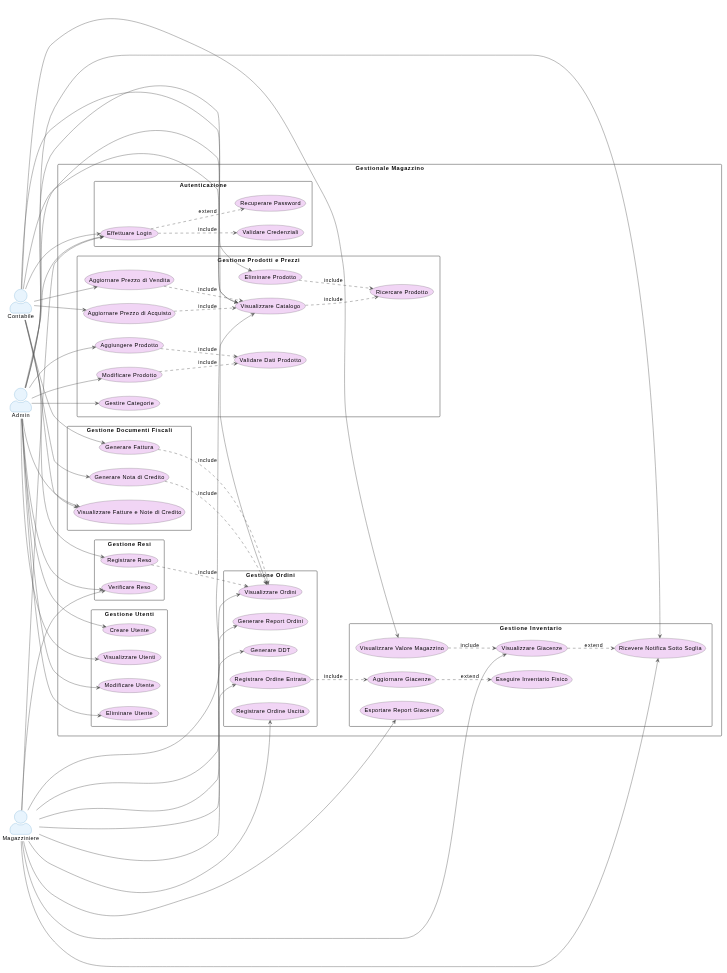
\includegraphics[width=\textwidth,height=0.82\textheight,keepaspectratio]{./img/UseCaseDiagram.png}
    \caption{Diagramma dei Casi d'Uso Generale}
\end{figure}
\clearpage

% ============================================================
\section{Progettazione e Architettura}
% ============================================================

\subsection{Scelte Architetturali}
Il sistema combina gli stili \emph{client--server}, \emph{layered} e \emph{repository}. Il client TUI \`{e} separato dal backend REST (Representational State Transfer) e comunica mediante HTTP (Hypertext Transfer Protocol) e JSON (JavaScript Object Notation). Nel server il router e il middleware costituiscono l'adattatore di trasporto; controller, service e repository separano rispettivamente conversione dei DTO, regole applicative e persistenza. Non si tratta di MVC (Model-View-Controller) classico: la View appartiene al processo client, mentre i controller del server sono controller HTTP.

\gialosaiNote{L'architettura client--server con TUI segue lo stesso pattern utilizzato da strumenti come \texttt{gh} (GitHub CLI) e \texttt{docker}: un client leggero che espone un'interfaccia testuale ricca, comunicando con un backend tramite API REST. Il pattern Repository \`{e} lo stesso adottato da \texttt{database/sql} in Go e da ORM (Object-Relational Mapping) come GORM, garantendo separazione tra logica applicativa e persistenza.}

I repository incapsulano query MySQL parametrizzate. I service dipendono da interfacce ristrette e sono quindi verificabili con mock, coerentemente con Dependency Inversion. \texttt{TransactionHelper} propaga la transazione nel contesto, garantendo atomicità per operazioni quali aggiornamento delle giacenze e registrazione degli ordini. MySQL 8, InnoDB e le chiavi esterne sono configurati nello script \texttt{docker/mysql/init.sql}.

\subsection{Modello del Dominio}
Il dominio dell'applicazione è incentrato sulle entità fondamentali per il tracciamento logistico, mappate nel file \texttt{Domain\_model.puml}: \texttt{Utente} e \texttt{Sessione}, \texttt{Categoria}, \texttt{Prodotto} e \texttt{Giacenza}, \texttt{OrdineEntrata} e \texttt{OrdineUscita} con le rispettive righe, \texttt{DDT}, \texttt{Fattura} (comprese le note di credito, distinte dal tipo) e \texttt{Reso}.

\clearpage
\begin{figure}[p]
    \centering
    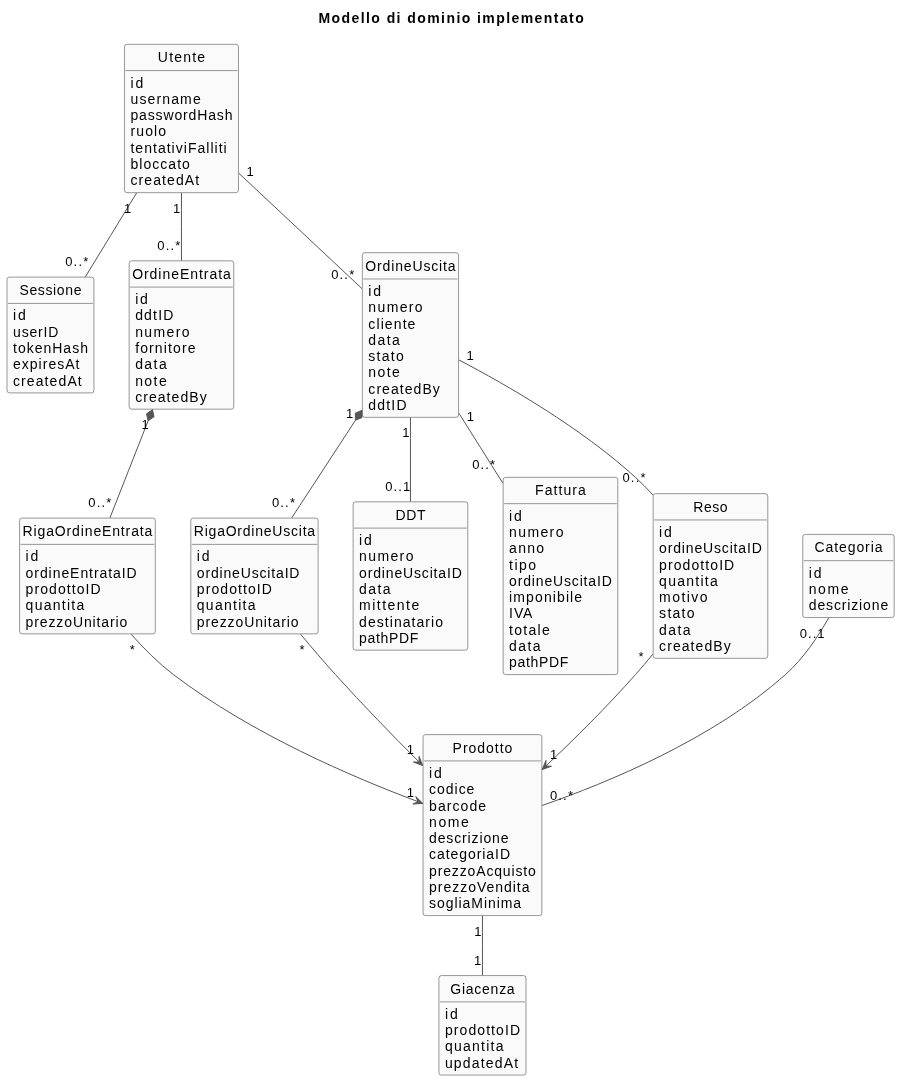
\includegraphics[width=\textwidth,height=0.82\textheight,keepaspectratio]{./img/DomainModel.png}
    \caption{Modello del Dominio}
\end{figure}
\clearpage

\subsection{Design Dettagliato (Diagramma delle Classi)}
Il modello del codice comprende entità di dominio, DTO, controller, service e repository. Il pattern Repository isola il dialetto SQL e il dettaglio della connessione dal service layer. L'aggregazione dei componenti avviene in \texttt{router.NewRouter}; il dominio rimane indipendente da HTTP e da MySQL. Il diagramma delle classi è una vista di design e deve essere letto insieme al codice: le operazioni effettivamente pubblicate sono determinate dalle rotte del router.

\clearpage
\begin{figure}[p]
    \centering
    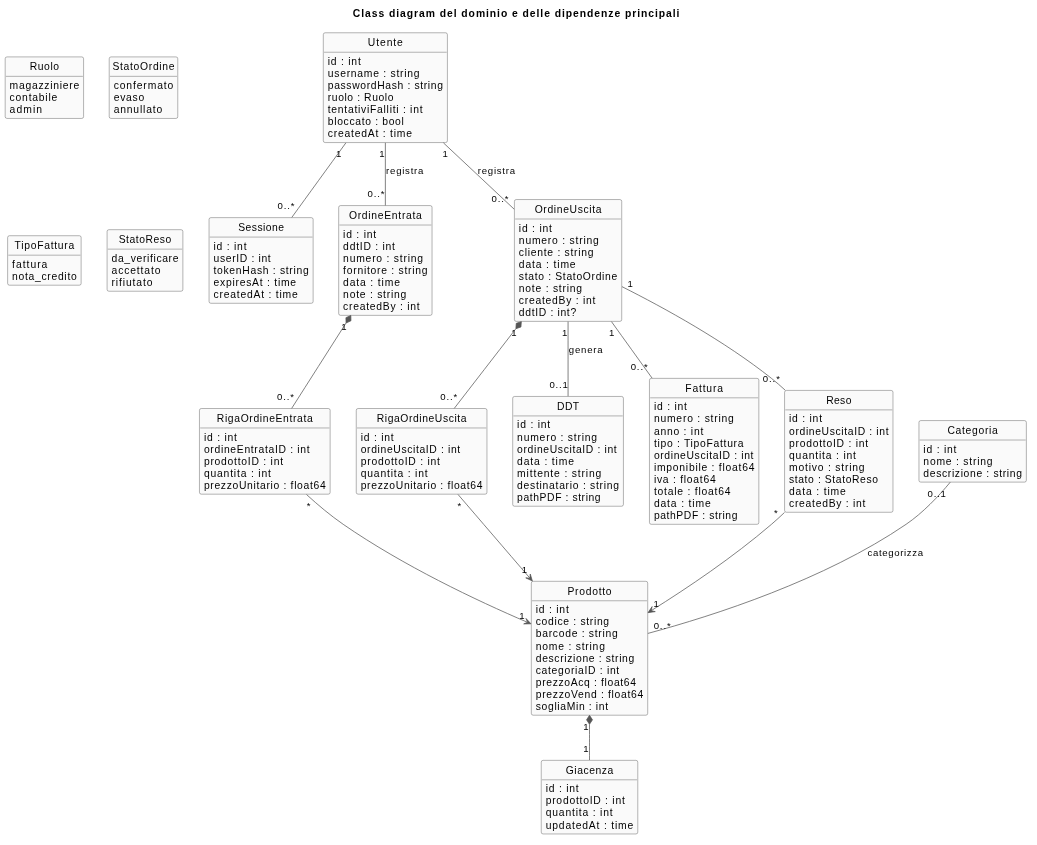
\includegraphics[width=\textwidth,height=0.82\textheight,keepaspectratio]{./img/ClassDiagram.png}
    \caption{Diagramma delle Classi}
\end{figure}
\clearpage

\subsection{Comportamento del Sistema (Diagrammi di Sequenza)}
I diagrammi rappresentano scenari di requisiti e design, e descrivono i flussi implementati nel codice. Login, catalogo, categorie, prezzi, ordini (entrata/uscita), DDT, fatture, note di credito e resi sono tutti esposti come rotte HTTP dal router, e le relative operazioni sono raggiungibili dalla navigazione TUI. I diagrammi sono quindi una vista di design allineata al codice; la disponibilità effettiva di ogni operazione resta comunque determinata dalle rotte del router e dalla navigazione della TUI.

\clearpage
\begin{figure}[p]
    \centering
    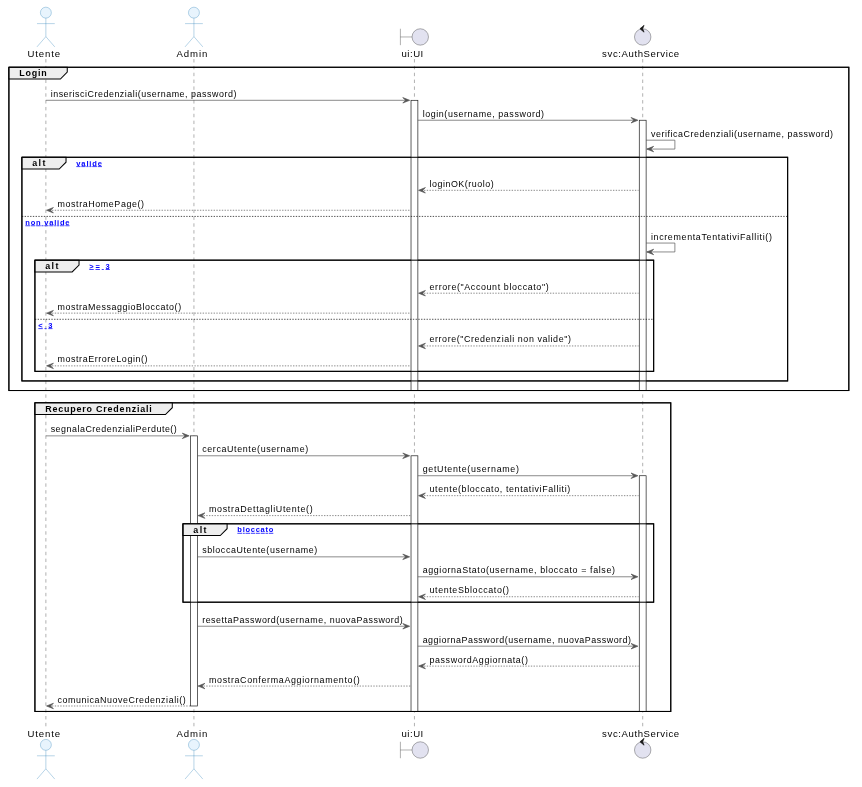
\includegraphics[width=\textwidth,height=0.82\textheight,keepaspectratio]{./img/UC1_SD.png}
    \caption{Diagramma di Sequenza: Login e Recupero Password (UC1)}
\end{figure}
\clearpage

\clearpage
\begin{figure}[p]
    \centering
    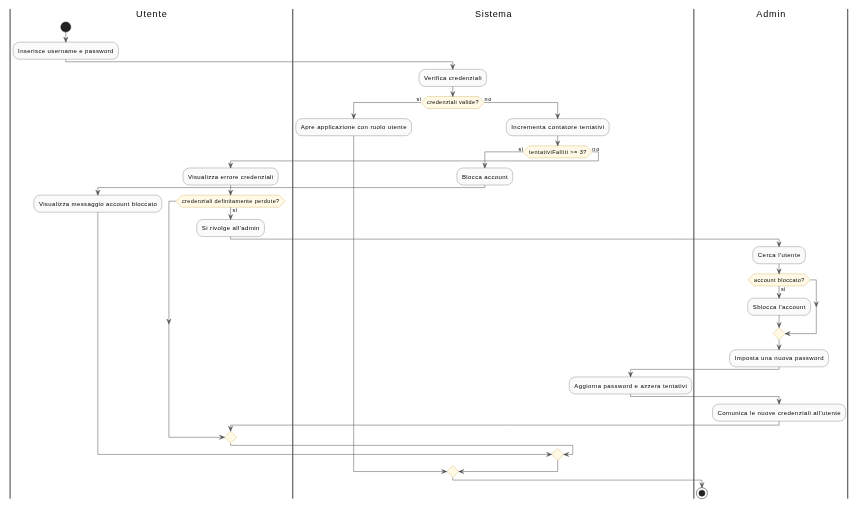
\includegraphics[width=\textwidth,height=0.82\textheight,keepaspectratio]{./img/UC1_AD.png}
    \caption{Diagramma di Attività: Login e Recupero Password (UC1)}
\end{figure}
\clearpage

\clearpage
\begin{figure}[p]
    \centering
    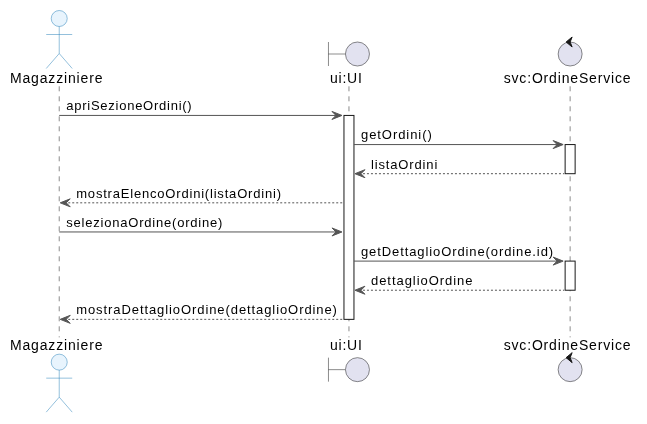
\includegraphics[width=\textwidth,height=0.82\textheight,keepaspectratio]{./img/UC2_SD.png}
    \caption{Diagramma di Sequenza: Visualizzazione Ordini (UC2)}
\end{figure}
\clearpage

\clearpage
\begin{figure}[p]
    \centering
    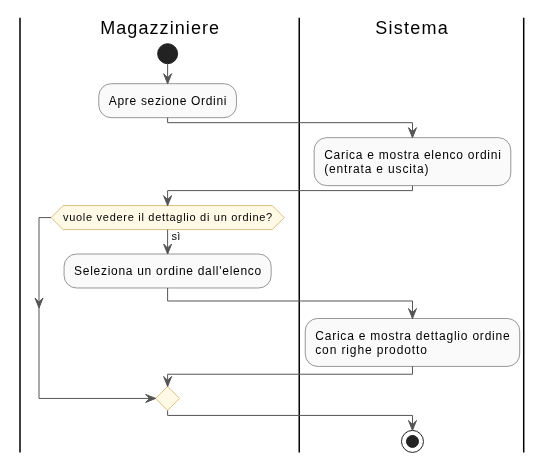
\includegraphics[width=\textwidth,height=0.82\textheight,keepaspectratio]{./img/UC2_AD.png}
    \caption{Diagramma di Attività: Visualizzazione Ordini (UC2)}
\end{figure}
\clearpage

\clearpage
\begin{figure}[p]
    \centering
    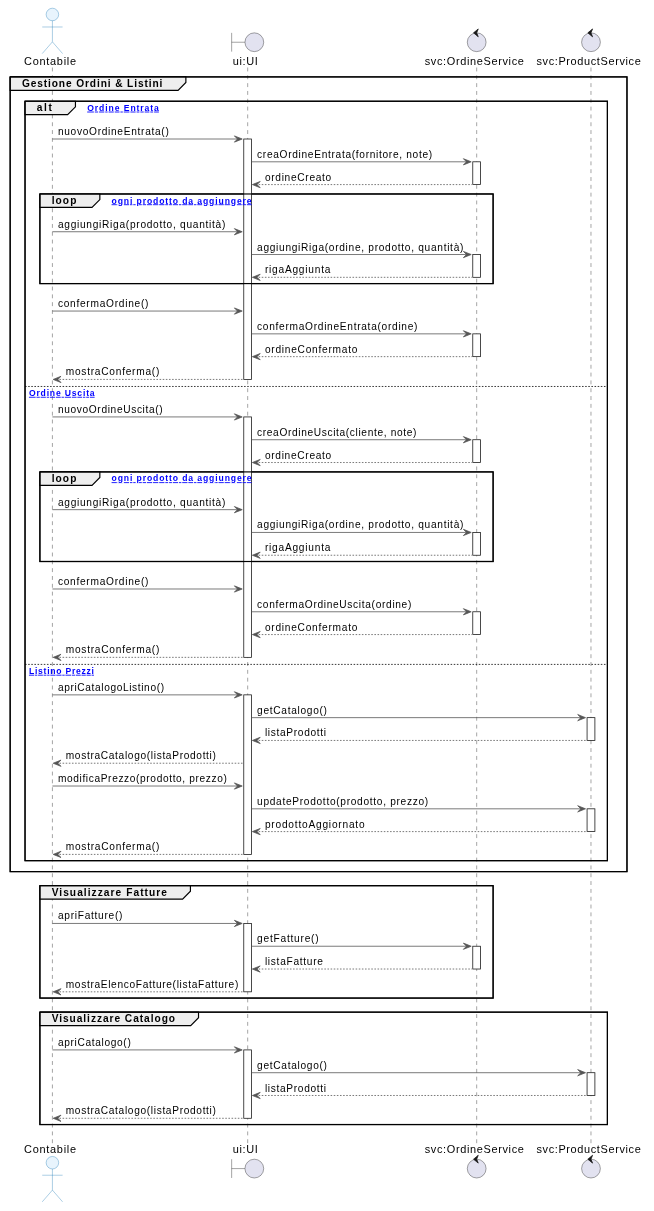
\includegraphics[width=\textwidth,height=0.82\textheight,keepaspectratio]{./img/UC3_SD.png}
    \caption{Diagramma di Sequenza: Gestione Ordini \& Listini (UC3)}
\end{figure}
\clearpage

\clearpage
\begin{figure}[p]
    \centering
    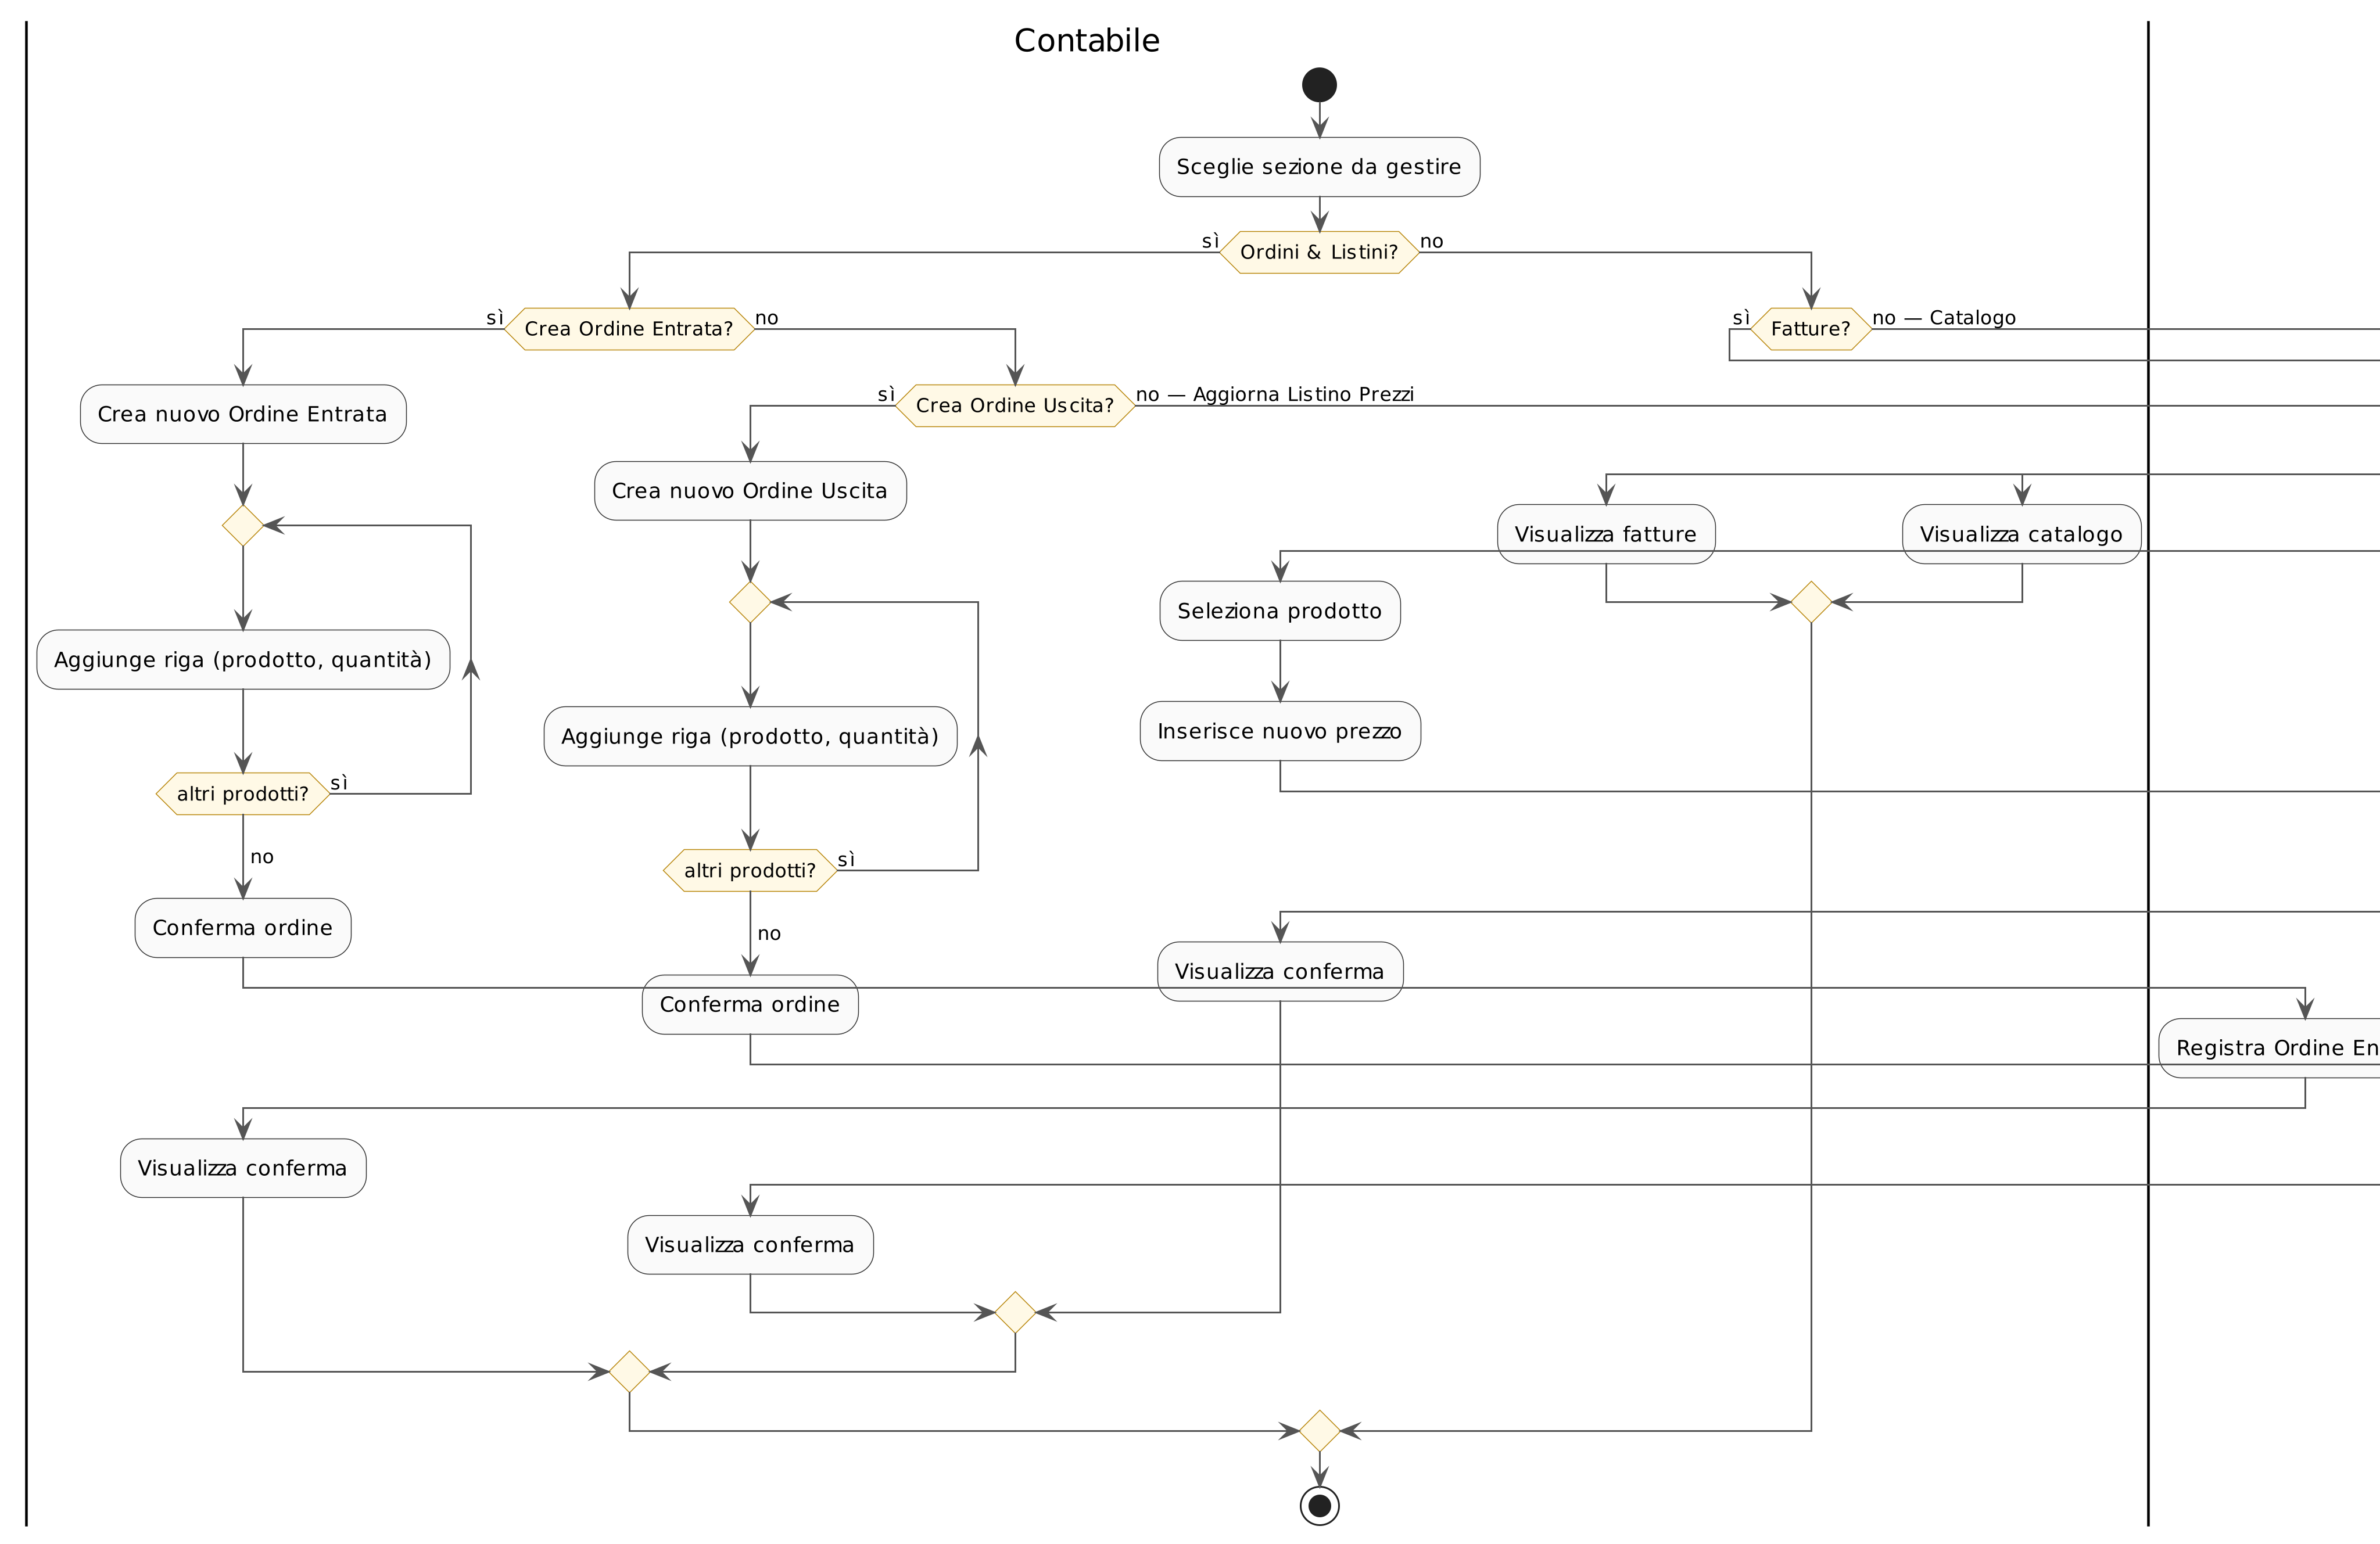
\includegraphics[width=\textwidth,height=0.82\textheight,keepaspectratio]{./img/UC3_AD.png}
    \caption{Diagramma di Attività: Gestione Ordini \& Listini (UC3)}
\end{figure}
\clearpage

\clearpage
\begin{figure}[p]
    \centering
    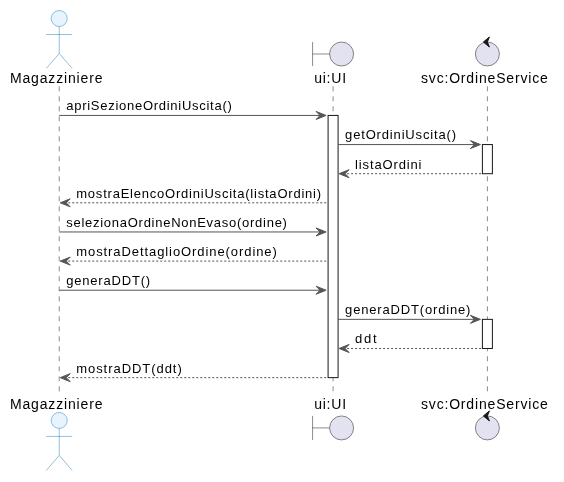
\includegraphics[width=\textwidth,height=0.82\textheight,keepaspectratio]{./img/UC4_SD.png}
    \caption{Diagramma di Sequenza: Generazione DDT (UC4)}
\end{figure}
\clearpage

\clearpage
\begin{figure}[p]
    \centering
    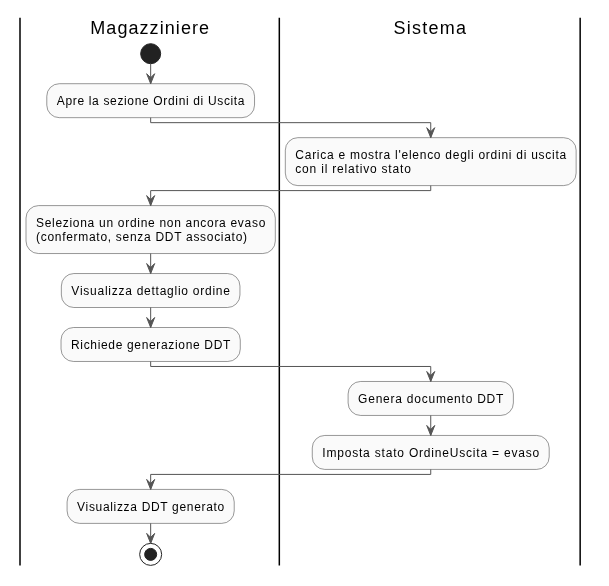
\includegraphics[width=\textwidth,height=0.82\textheight,keepaspectratio]{./img/UC4_AD.png}
    \caption{Diagramma di Attività: Generazione DDT (UC4)}
\end{figure}
\clearpage

\clearpage
\begin{figure}[p]
    \centering
    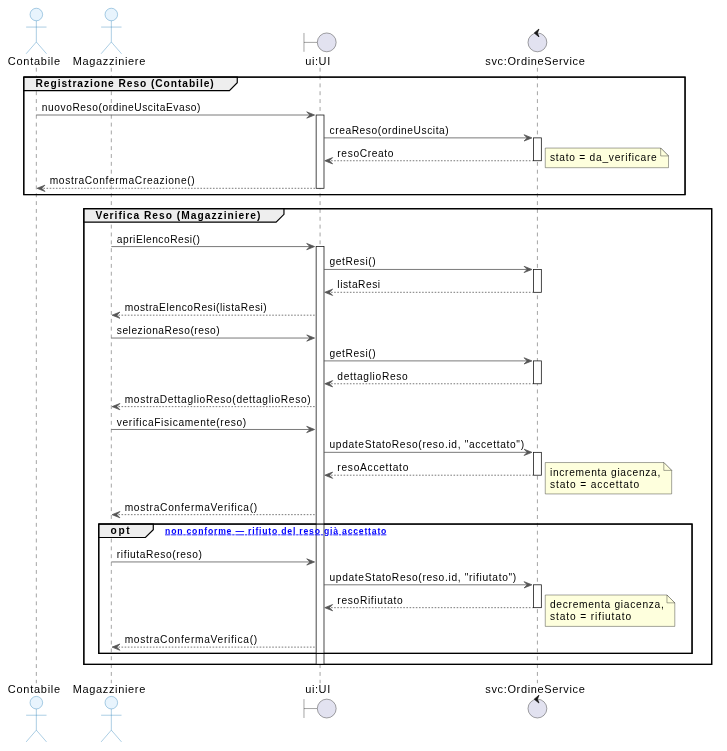
\includegraphics[width=\textwidth,height=0.82\textheight,keepaspectratio]{./img/UC5_SD.png}
    \caption{Diagramma di Sequenza: Resi (UC5)}
\end{figure}
\clearpage

\clearpage
\begin{figure}[p]
    \centering
    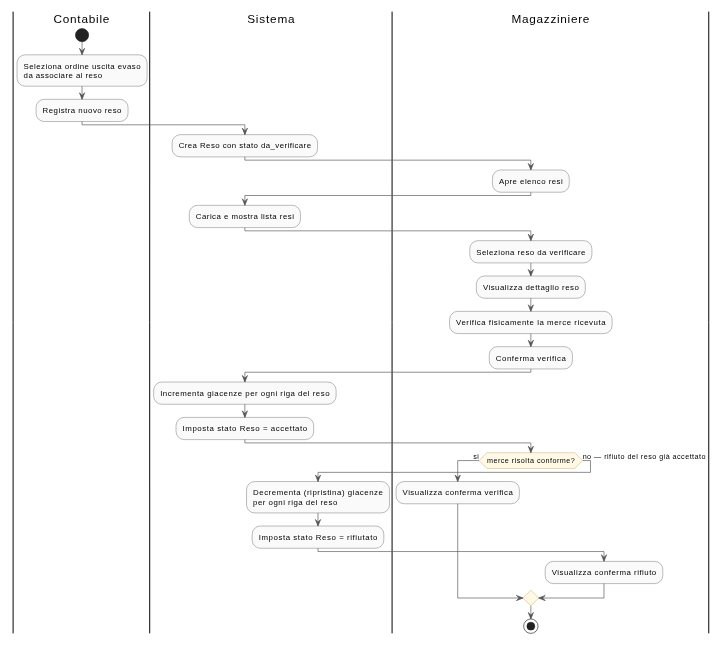
\includegraphics[width=\textwidth,height=0.82\textheight,keepaspectratio]{./img/UC5_AD.png}
    \caption{Diagramma di Attività: Resi (UC5)}
\end{figure}
\clearpage

\clearpage
\begin{figure}[p]
    \centering
    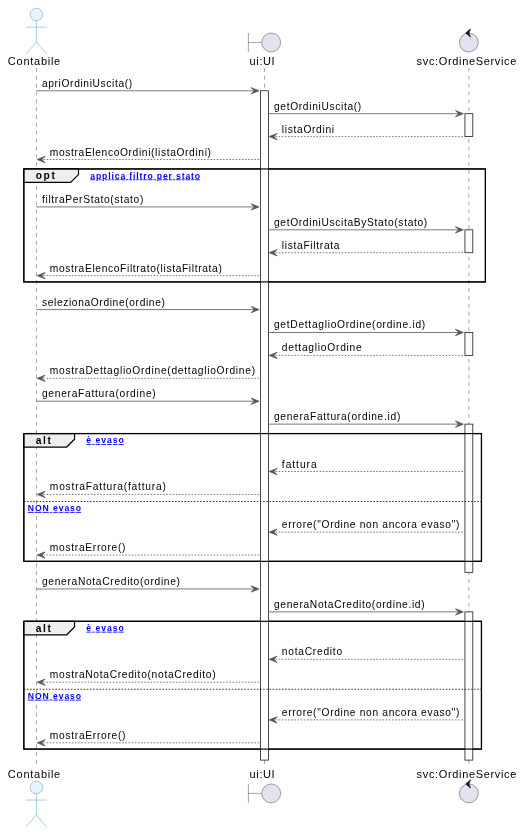
\includegraphics[width=\textwidth,height=0.82\textheight,keepaspectratio]{./img/UC6_SD.png}
    \caption{Diagramma di Sequenza: Contabile Ordini (UC6)}
\end{figure}
\clearpage

\clearpage
\begin{figure}[p]
    \centering
    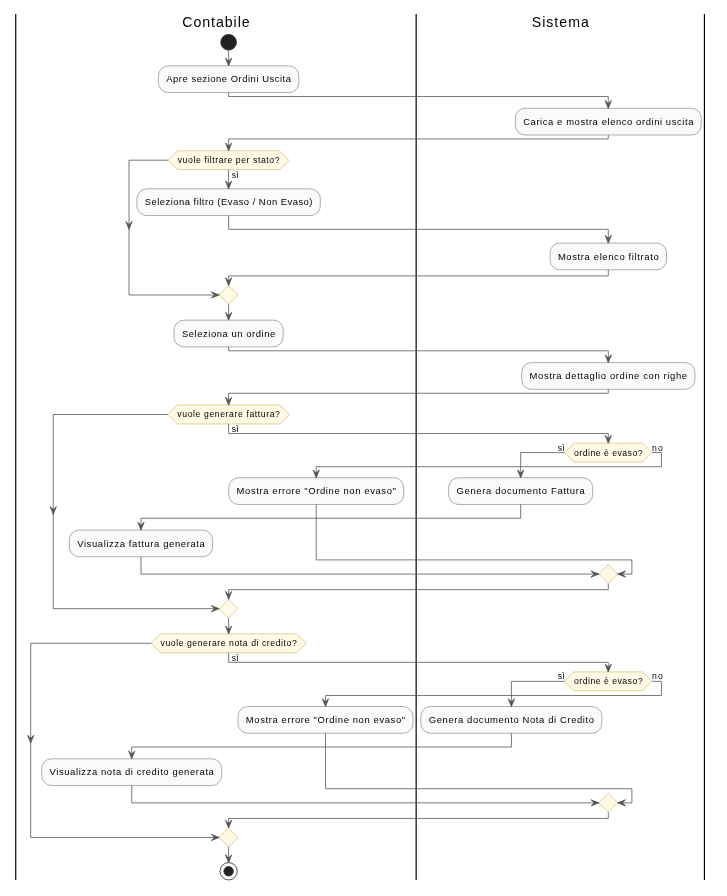
\includegraphics[width=\textwidth,height=0.82\textheight,keepaspectratio]{./img/UC6_AD.png}
    \caption{Diagramma di Attività: Contabile Ordini (UC6)}
\end{figure}
\clearpage

\clearpage
\begin{figure}[p]
    \centering
    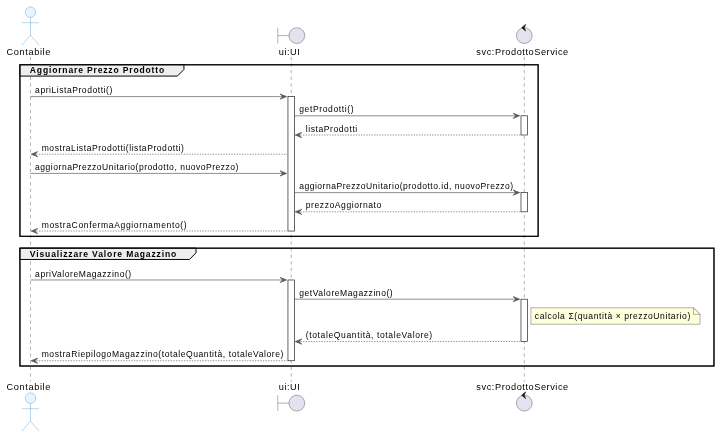
\includegraphics[width=\textwidth,height=0.82\textheight,keepaspectratio]{./img/UC7_SD.png}
    \caption{Diagramma di Sequenza: Contabile Prezzi (UC7)}
\end{figure}
\clearpage

\clearpage
\begin{figure}[p]
    \centering
    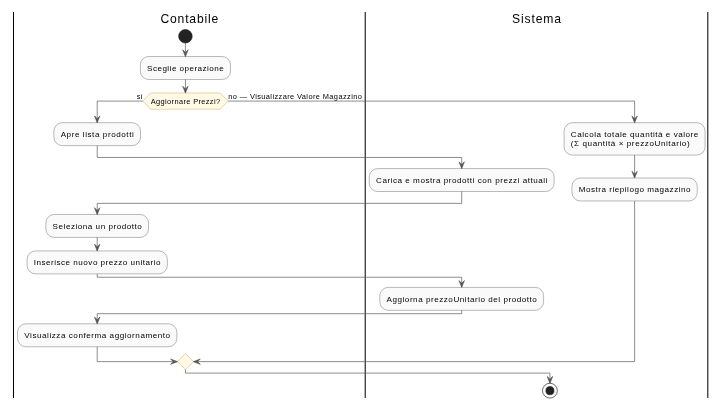
\includegraphics[width=\textwidth,height=0.82\textheight,keepaspectratio]{./img/UC7_AD.png}
    \caption{Diagramma di Attività: Contabile Prezzi (UC7)}
\end{figure}
\clearpage

\clearpage
\begin{figure}[p]
    \centering
    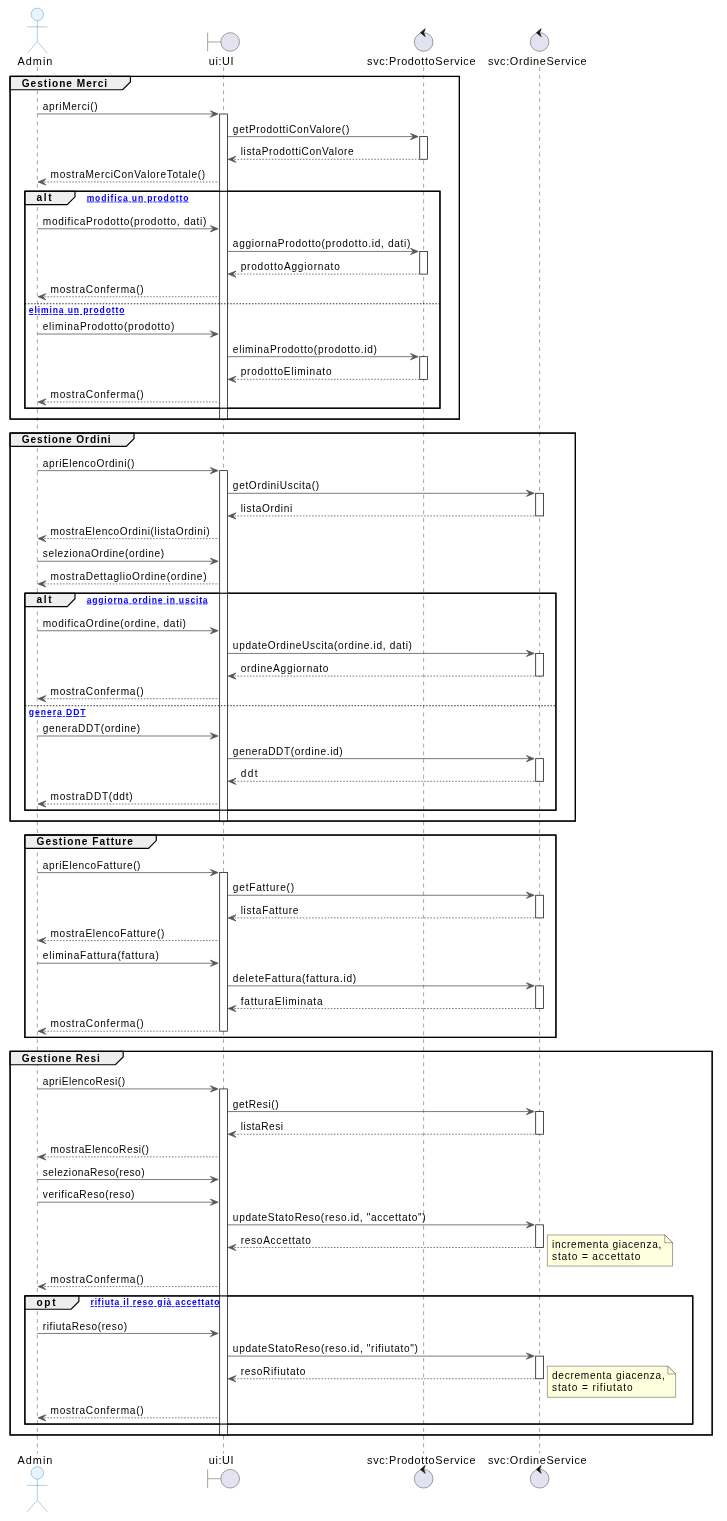
\includegraphics[width=\textwidth,height=0.82\textheight,keepaspectratio]{./img/UC8_SD.png}
    \caption{Diagramma di Sequenza: Admin (UC8)}
\end{figure}
\clearpage

\clearpage
\begin{figure}[p]
    \centering
    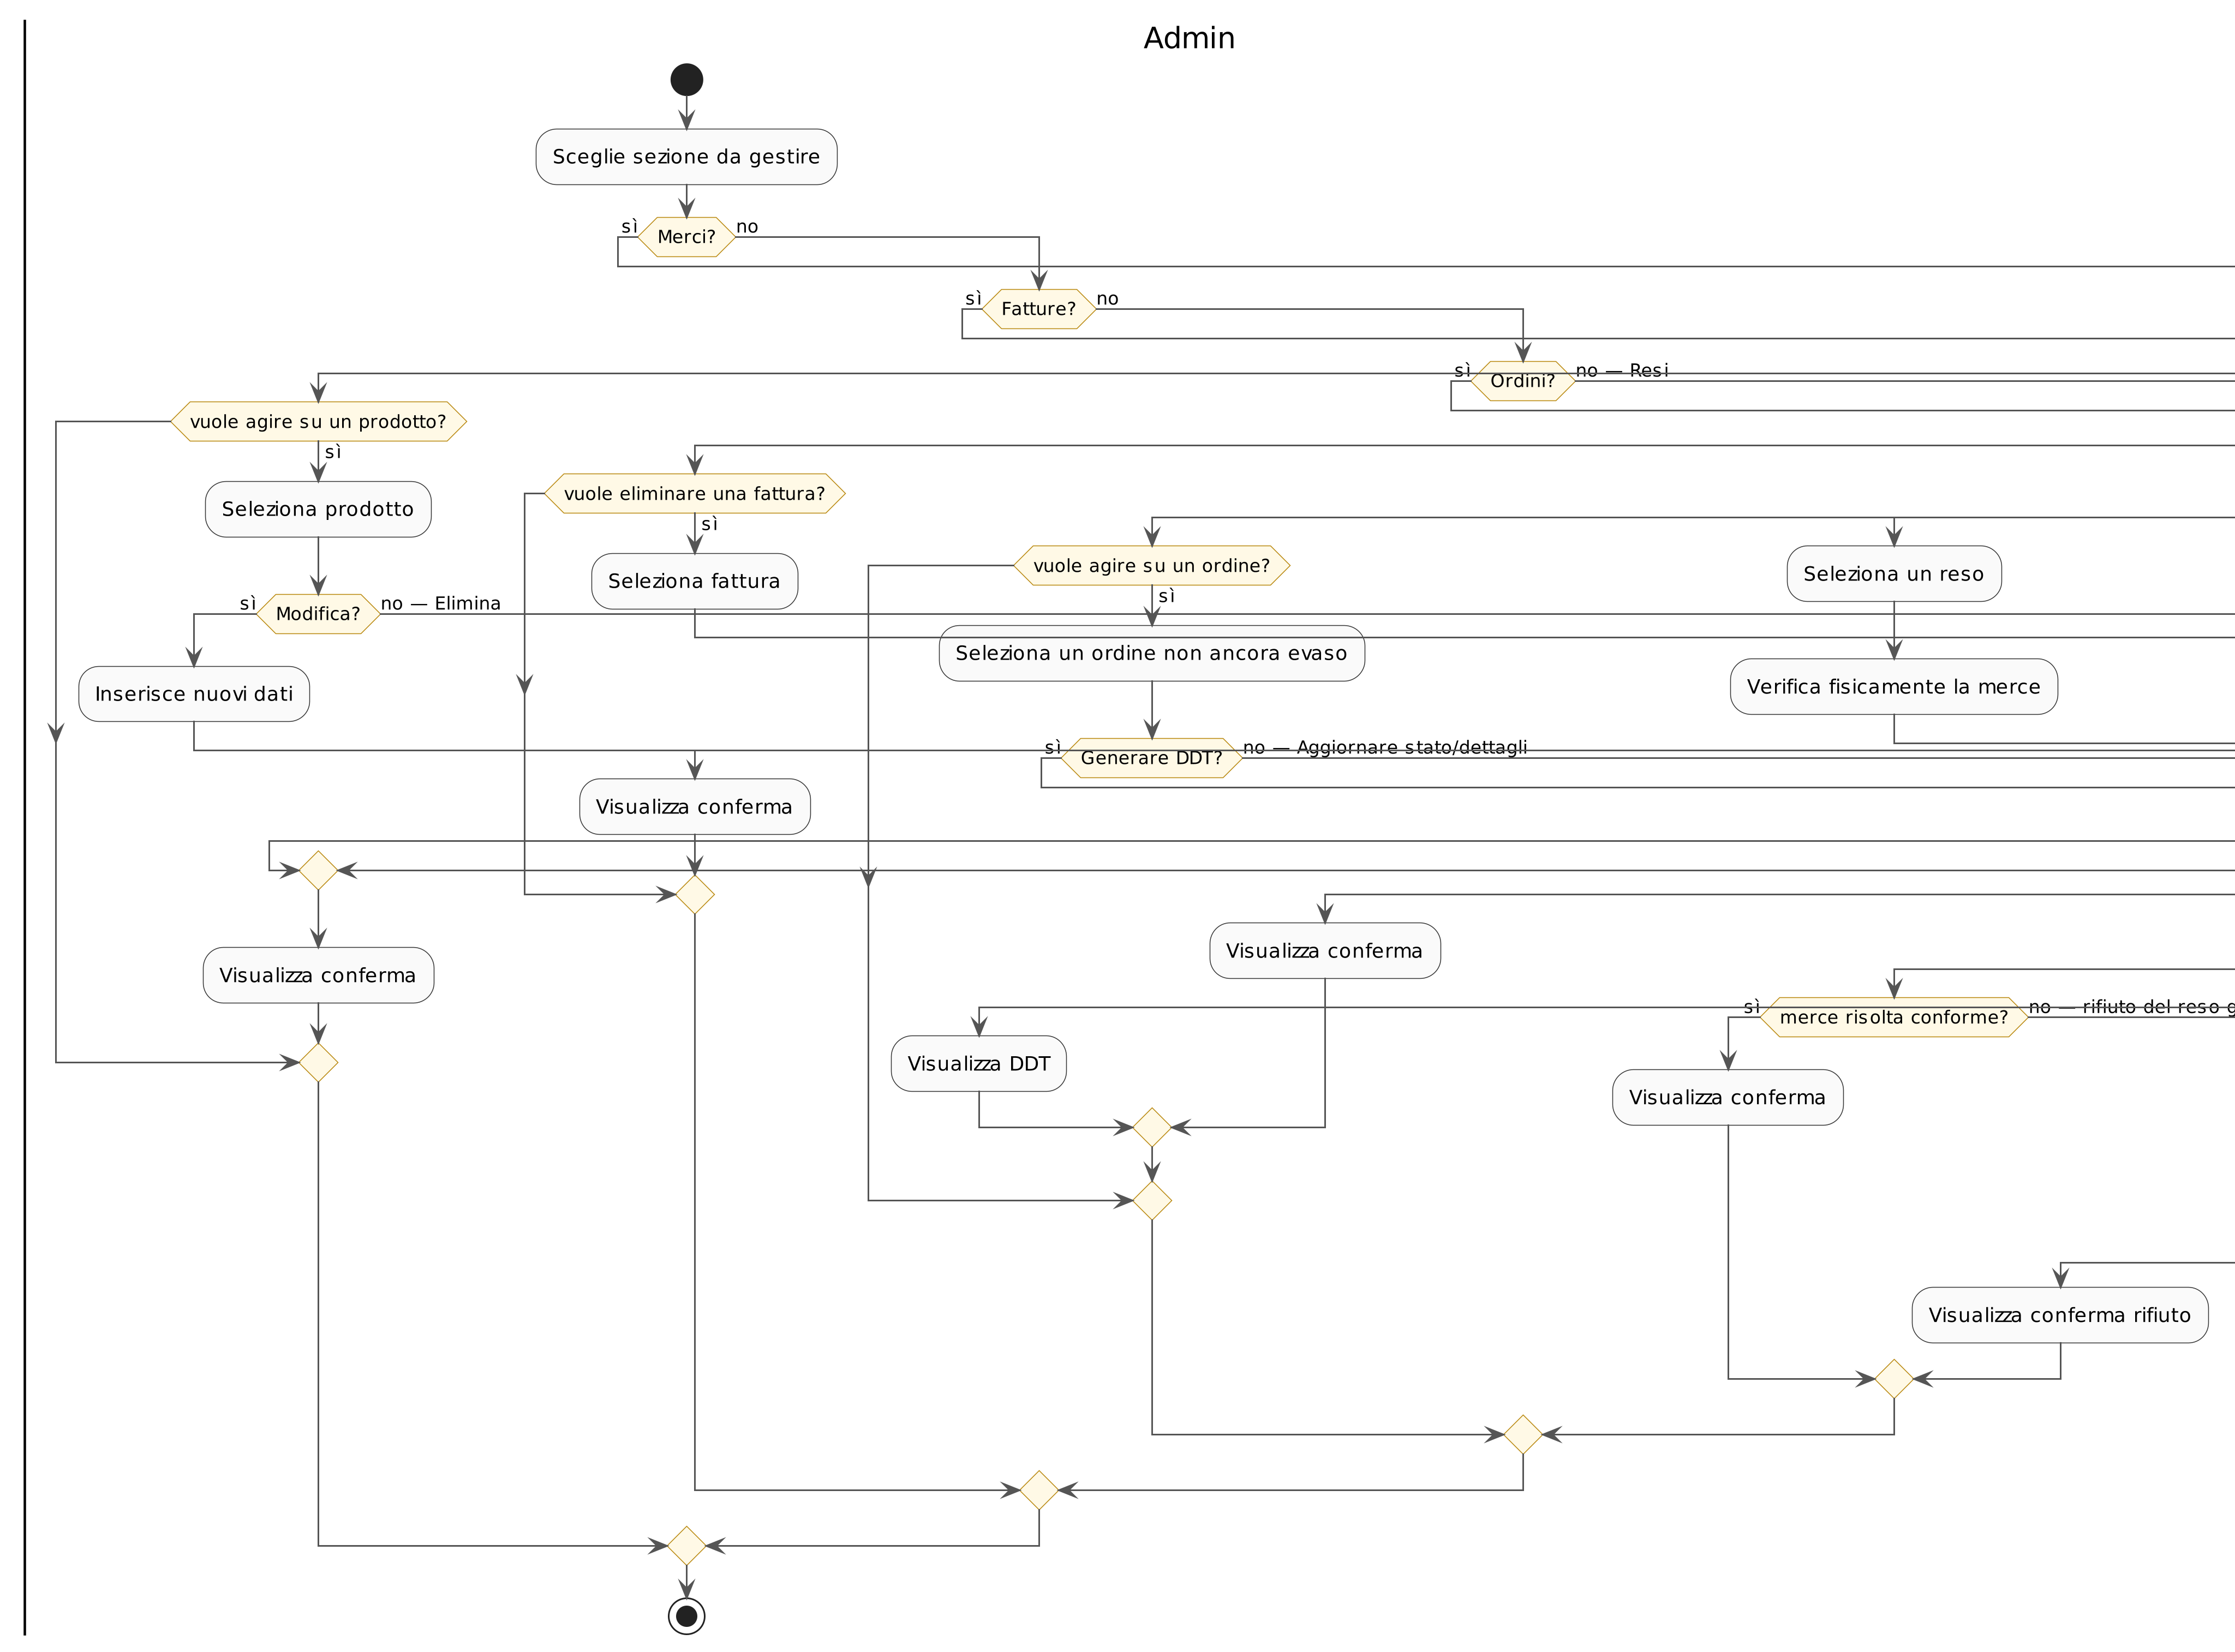
\includegraphics[width=\textwidth,height=0.82\textheight,keepaspectratio]{./img/UC8_AD.png}
    \caption{Diagramma di Attività: Admin (UC8)}
\end{figure}
\clearpage

\clearpage
\begin{figure}[p]
    \centering
    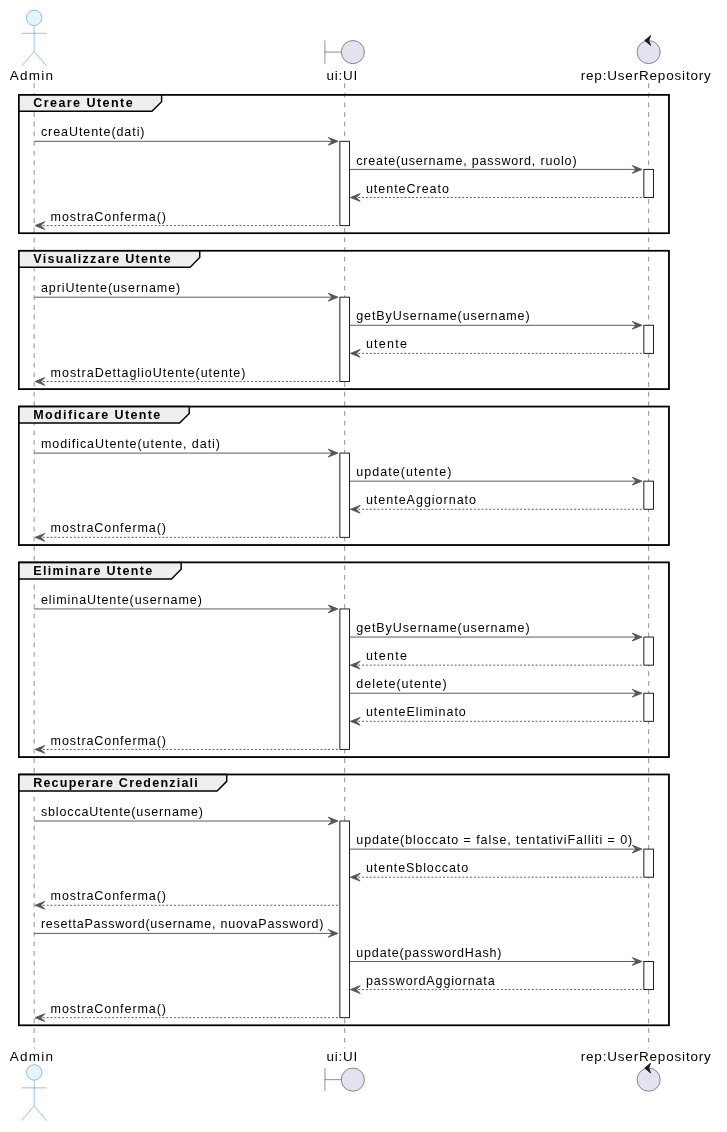
\includegraphics[width=\textwidth,height=0.82\textheight,keepaspectratio]{./img/UC9_SD.png}
    \caption{Diagramma di Sequenza: Gestione Utenti (UC9)}
\end{figure}
\clearpage

\clearpage
\begin{figure}[p]
    \centering
    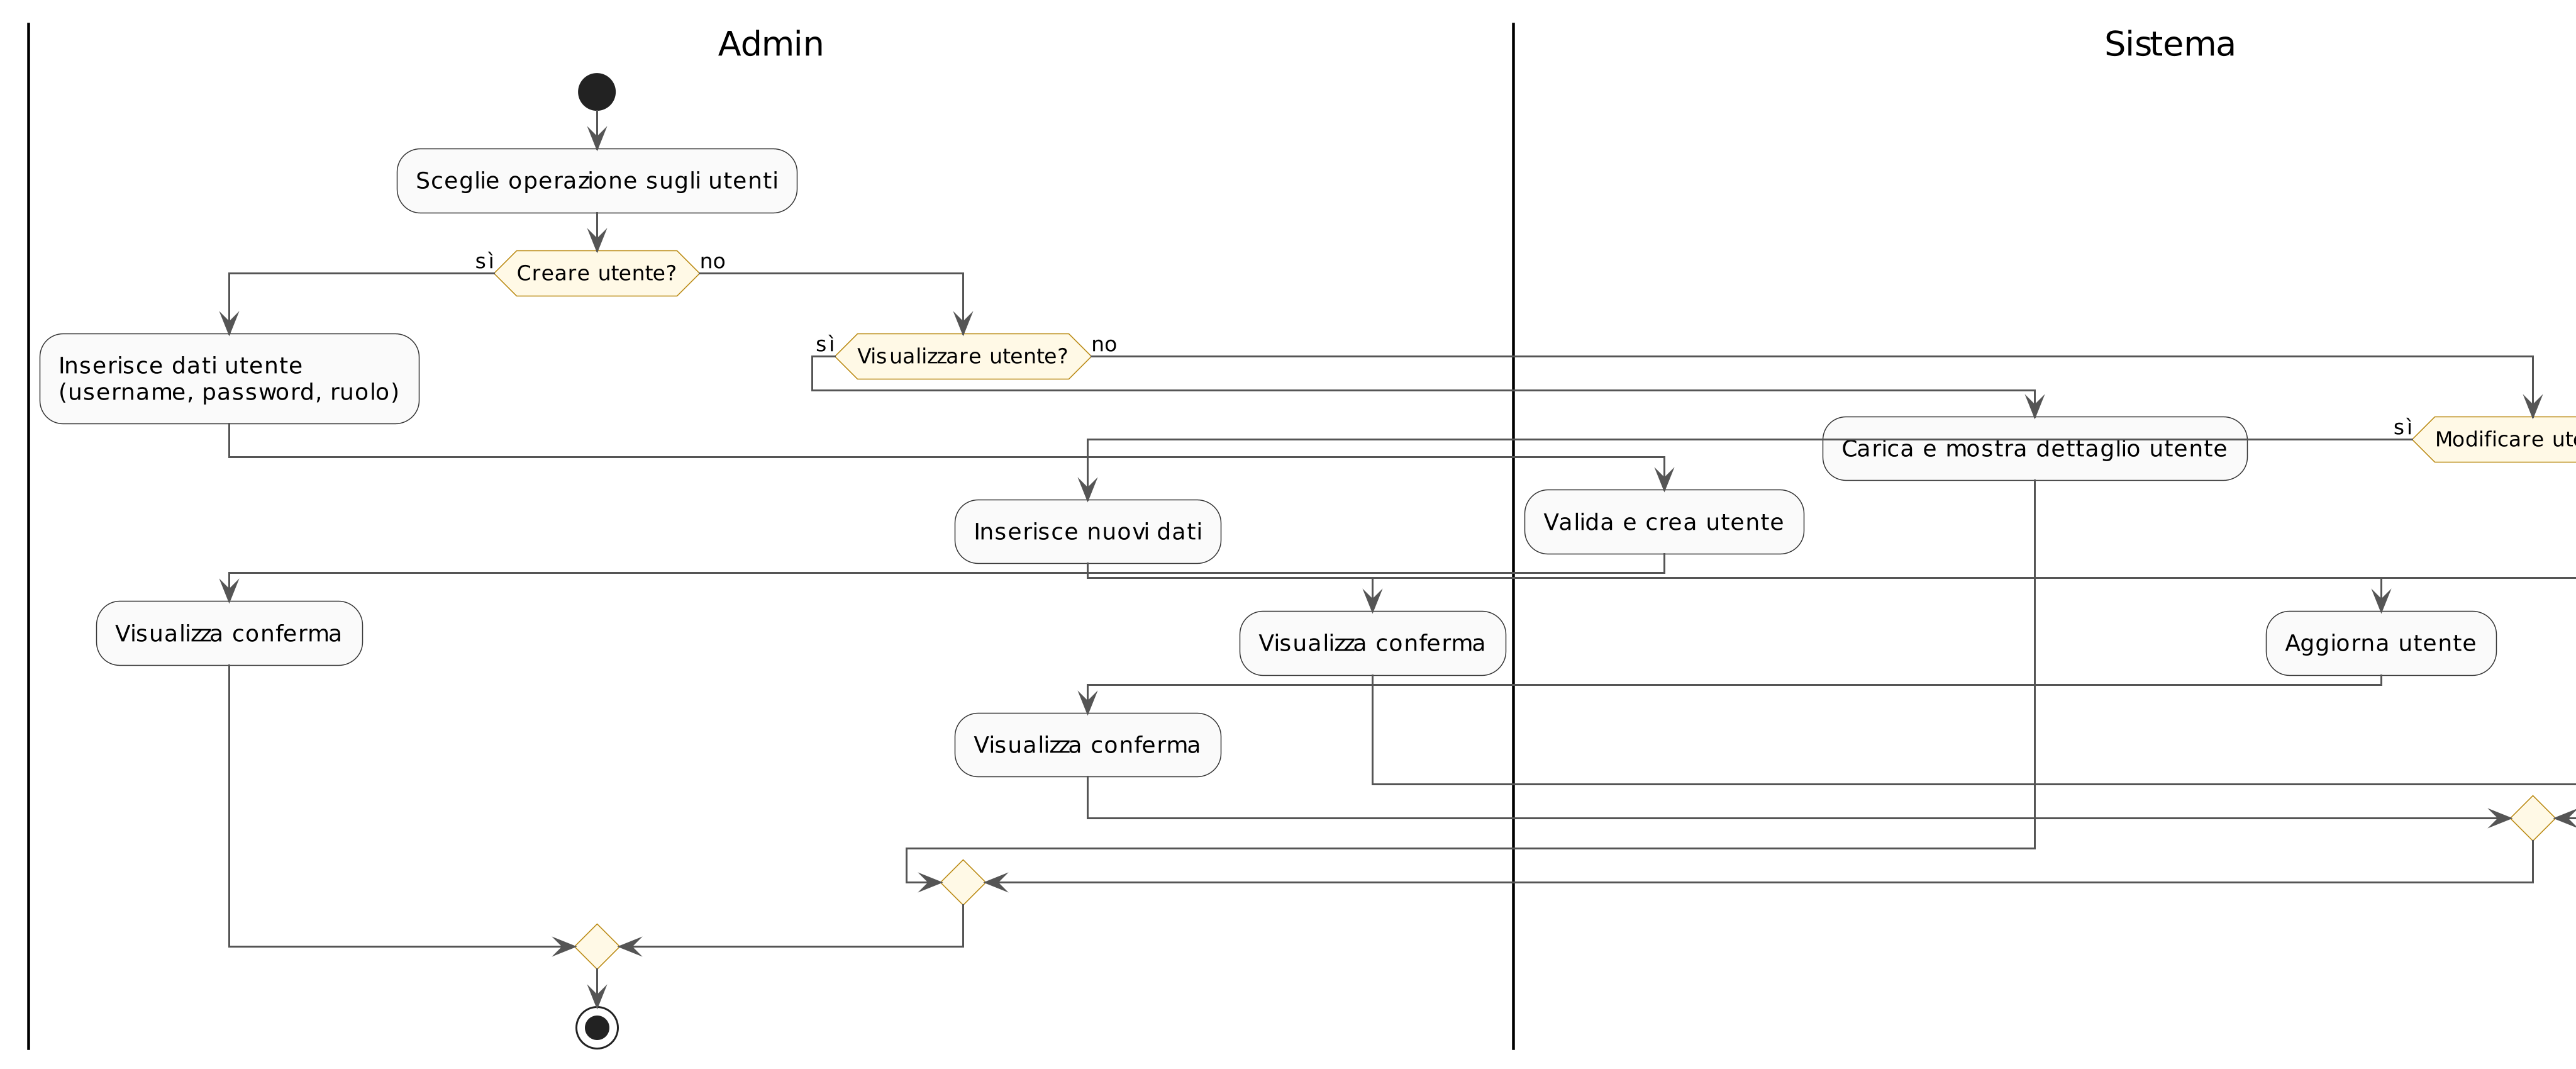
\includegraphics[width=\textwidth,height=0.82\textheight,keepaspectratio]{./img/UC9_AD.png}
    \caption{Diagramma di Attività: Gestione Utenti (UC9)}
\end{figure}
\clearpage

% ============================================================
\section{Gestione del Progetto (Scrum)}
% ============================================================

\subsection{Backlog}
L'elenco ordinato e prioritizzato dei requisiti tecnici necessari al completamento del primo ciclo di sviluppo comprende:
\begin{enumerate}
    \item Configurazione dell'architettura software di base, dell'ambiente Docker e della connessione a MySQL.
    \item Definizione dello schema logico della base dati tramite script SQL (creazione delle tabelle \texttt{Utente}, \texttt{Prodotto}, \texttt{Categoria}, \texttt{Giacenza}, \texttt{OrdineEntrata}, \texttt{OrdineUscita}, \texttt{RigaOrdineEntrata}, \texttt{RigaOrdineUscita}, \texttt{DDT}).
    \item Sviluppo delle interfacce grafiche e delle funzioni CRUD (Create, Read, Update, Delete) per la gestione dell'Anagrafica Prodotti e Categorie.
    \item Implementazione del modulo di movimentazione (logica e maschere per la compilazione di \texttt{OrdineEntrata} e \texttt{OrdineUscita}).
    \item Integrazione software per l'acquisizione dell'input da lettore di codici a barre tramite emulazione tastiera.
    \item Sviluppo del sottosistema di controllo e notifica visiva per i prodotti sotto la soglia minima inseriti in \texttt{Giacenza}.
    \item Sviluppo del modulo di autenticazione locale e gestione dei permessi basata sui ruoli tramite \texttt{AuthService}.
\end{enumerate}

\subsection{User Stories}
Le storie riflettono i bisogni concreti degli attori scritti secondo gli standard del framework Scrum:
\begin{itemize}
    \item \textbf{US-01 (Accesso con credenziali)}: "Come utente, voglio accedere all'applicazione con username e password, in modo da poter utilizzare le funzionalità del mio ruolo".
    \item \textbf{US-02 (Scansione Barcode)}: "Come magazziniere, voglio poter scansionare il codice a barre di un prodotto in arrivo tramite il lettore ottico, per aggiornare la quantità in giacenza nel sistema in modo rapido, automatizzato e senza commettere errori manuali".
    \item \textbf{US-03 (Sicurezza Account)}: "Come admin del sistema, voglio che il software blocchi l'account dopo 3 tentativi falliti, per impedire ad utenti non autorizzati di indovinare le password d'accesso dei dipendenti".
    \item \textbf{US-04 (Recupero Credenziali)}: "Come admin, voglio poter sbloccare eventuali utenti bloccati, per consentire loro di accedere nuovamente all'applicazione".
    \item \textbf{US-05 (Visualizzazione elenco ordini)}: "Come magazziniere, voglio vedere l'elenco di tutti gli ordini di entrata e uscita, in modo da avere una panoramica completa dei movimenti del magazzino".
    \item \textbf{US-06 (Visualizzazione dettaglio ordini)}: "Come magazziniere, voglio vedere il dettaglio di un ordine di entrata o uscita selezionato, in modo da conoscere i prodotti coinvolti e le relative quantità".
    \item \textbf{US-07 (Registrazione Ordini in entrata)}: "Come contabile, voglio registrare un ordine di entrata con i prodotti ricevuti, in modo da aggiornare automaticamente le giacenze".
    \item \textbf{US-08 (Registrazione Ordini in uscita)}: "Come contabile, voglio registrare un ordine di uscita con i prodotti richiesti, in modo da aggiornare automaticamente le giacenze".
    \item \textbf{US-09 (Generazione DDT)}: "Come magazziniere, voglio generare un documento di trasporto (DDT) per ogni ordine di uscita evaso, in modo da modificarne lo stato eavere una documentazione ufficiale per la merce in uscita".
    \item \textbf{US-10 (Visualizzare Giacenze)}: "Come magazziniere, voglio visualizzare in tempo reale le giacenze di magazzino, in modo da sapere sempre la quantità disponibile di ogni prodotto".
    \item \textbf{US-11 (Creazione resi)}: "Come contabile, voglio generare le pratiche di reso della merce, in modo da poter operare correttamente i resi".
    \item \textbf{US-12 (Visualizzazione ordini per contabile)}: "Come contabile, voglio visualizzare l'elenco degli ordini ricevuti (evasi e non evasi), in modo da poter gestire la fatturazione e le note di credito".
    \item \textbf{US-13 (Generazione Fatture)}: "Come contabile, voglio generare fatture per gli ordini di uscita evasi, in modo da poter emettere documenti ufficiali per i clienti".
    \item \textbf{US-14 (Nota di credito)}: "Come contabile, voglio generare una nota di credito per un ordine di uscita evaso, in modo da correggere la fatturazione quando necessario".
    \item \textbf{US-15 (Gestione prezzi)}: "Come contabile, voglio poter modificare manualmente i listini dei prezzi di vendita e di acquisto dei prodotti, in modo da mantenere aggiornati i prezzi nel sistema".
    \item \textbf{US-16 (Gestione utenti)}: "Come admin, voglio creare, modificare ed eliminare gli account degli utenti, in modo da gestire l'accesso al sistema e i relativi ruoli".
    \item \textbf{US-17 (Reportistica inventario)}: "Come contabile, voglio visualizzare report avanzati dell'inventario, in modo da avere una visione dettagliata dello stato del magazzino e delle tendenze di consumo dei prodotti".
    \item \textbf{US-18 (Modifica stato reso)}: "Come magazziniere, voglio poter modificare lo stato di un reso, in modo da aggiornare correttamente le giacence e la documentazione associata".
    \item \textbf{US-19 (Accesso privilegiato)}: "Come admin, voglio poter avere accesso alle funzioni riservate agli altri tipi di utenti, in modo da poter supervisionare e gestire l'intero sistema".
\end{itemize}

\gialosaiNote{Per le fatture e le note di credito (RF-13) l'importo mostrato è calcolato a partire dalle righe dell'ordine come \emph{totale}, cioè imponibile più IVA al \textbf{22\%}: $\texttt{totale} = \texttt{imponibile} + (\texttt{imponibile} \times 0.22)$, con $\texttt{imponibile} = \sum_{riga}(\texttt{quantita} \times \texttt{prezzo\_unitario})$. Il valore visualizzato nella TUI è quindi \emph{prezzo + 22\% di IVA}.}

\subsection{Criteri di Accettazione}
Vengono definiti i vincoli formali affinché ciascuna User Story possa essere considerata completata (``Done''). I criteri sono organizzati per area funzionale, a partire dalle principali storie del progetto.

\subsubsection*{Autenticazione e Sicurezza (US-01, US-03, US-04)}
\begin{itemize}
    \item \textbf{US-01 -- Accesso con credenziali}: il sistema deve accettare il login solo con username e password validi; in caso di successo deve restituire un token JWT e il ruolo dell'utente, e deve inoltrare l'utente alla home del proprio ruolo.
    \item \textbf{US-03 -- Sicurezza Account}: dopo 3 tentativi di login falliti consecutivi l'account deve essere bloccato automaticamente, con l'eccezione dell'account \texttt{admin}; un account bloccato non deve poter autenticarsi.
    \item \textbf{US-04 -- Recupero Credenziali}: l'admin deve poter sbloccare un account bloccato (con azzeramento dei tentativi falliti) e reimpostarne la password; il ripristino deve essere registrato nel database.
\end{itemize}

\subsubsection*{Prodotti e Giacenze (US-02, US-10)}
\begin{itemize}
    \item \textbf{US-02 -- Scansione Barcode}: il sistema deve riconoscere e decodificare correttamente e senza latenza i codici a barre conformi allo standard internazionale EAN-13. Al momento della scansione riuscita all'interno della schermata di carico, i dati identificativi del prodotto devono comparire istantaneamente. Qualora il codice non trovi corrispondenza in \texttt{Prodotti}, il service restituisce un errore di prodotto non trovato. Feedback acustico, pop-up e inserimento contestuale non sono implementati nella TUI corrente.
    \item \textbf{US-10 -- Visualizzare Giacenze}: l'elenco delle giacenze deve mostrare per ogni prodotto la quantit\`{a} disponibile e segnalare visivamente i prodotti sotto la soglia minima di sicurezza, aggiornando i valori in tempo reale.
\end{itemize}

\subsubsection*{Ordini (US-05, US-06, US-07, US-08)}
\begin{itemize}
    \item \textbf{US-05/06 -- Visualizzare ordini}: il sistema deve mostrare l'elenco degli ordini di entrata e uscita e consentire di visualizzare il dettaglio di un ordine selezionato, con le righe prodotto e le relative quantit\`{a}.
    \item \textbf{US-07/08 -- Registrare ordini}: la registrazione di un ordine di entrata deve incrementare le giacenze dei prodotti coinvolti; la registrazione di un ordine di uscita deve verificare la disponibilit\`{a} e decrementare le giacenze. Se la quantit\`{a} richiesta supera la giacenza disponibile, la transazione deve annullarsi e restituire un errore di giacenza insufficiente.
\end{itemize}

\subsubsection*{Documenti e Contabilit\`{a} (US-09, US-12, US-13, US-14, US-15)}
\begin{itemize}
    \item \textbf{US-09 -- Generazione DDT}: la generazione di un DDT deve essere possibile solo per ordini di uscita confermati e deve portare automaticamente lo stato dell'ordine a ``Evaso''.
    \item \textbf{US-12 -- Ordini per il contabile}: il contabile deve poter visualizzare gli ordini di uscita, distinguendo quelli evasi da quelli non evasi.
    \item \textbf{US-13/14 -- Fatture e note di credito}: la generazione deve essere possibile solo per ordini di uscita nello stato ``Evaso'' e deve calcolare correttamente imponibile, IVA (22\%) e totale, assegnando una numerazione progressiva annuale.
    \item \textbf{US-15 -- Gestione prezzi}: la modifica del prezzo di vendita o di acquisto di un prodotto deve essere persistita nel database e riflessa nelle viste successive del catalogo.
\end{itemize}

\subsubsection*{Resi, Utenti e Reportistica (US-11, US-16, US-17)}
\begin{itemize}
    \item \textbf{US-11 -- Gestione resi}: la registrazione di un reso deve creare il reso con stato ``da\_verificare''; alla verifica, lo stato deve passare a ``accettato'' o ``rifiutato''.
    \item \textbf{US-16 -- Gestione utenti}: l'admin deve poter creare, visualizzare, modificare ed eliminare gli account utente; il sistema deve impedire la cancellazione di account con ordini a esso associati.
    \item \textbf{US-17 -- Reportistica inventario}: il report deve includere per ogni prodotto giacenza, soglia minima e stato di sotto-soglia, restituito in formato JSON dal router.
\end{itemize}

% ============================================================
\section{Strategia di Verifica e Validazione}
% ============================================================

\subsection{Piano di Testing}
Il piano prevede una suite di test di unità (Unit Testing) sistematici eseguiti sulla Business Logic tramite lo strumento standard di testing di Go (\texttt{go test}). I test sono focalizzati sulla verifica delle transazioni e sul rispetto dei vincoli di integrità del magazzino.

Oltre ai test di unità, la cartella \texttt{server/router/} contiene una suite di \emph{test di integrazione end-to-end} (\texttt{integration\_test.go}, 17 casi) che attraversano l'intera catena HTTP $\rightarrow$ router $\rightarrow$ middleware $\rightarrow$ controller $\rightarrow$ service $\rightarrow$ repository, con database mockato tramite \texttt{go-sqlmock}. Questi test verificano il contratto tra frontend e backend: path e metodo HTTP, status code e forma del body JSON, esattamente come il client TUI li attende quando comunica con il server reale.

\subsection{Casi di Test (Test Cases)}
\textbf{TC-01}: Tentativo di scarico merce con quantità richiesta superiore alla giacenza fisica attuale.
\begin{itemize}
    \item \textbf{Scenario}: Un prodotto registrato in anagrafica dispone di una quantità fisica in \texttt{Giacenza} pari a 5 unità. Viene inserito un \texttt{OrdineUscita} con una \texttt{RigaOrdineUscita} richiedente l'uscita di 6 unità del medesimo prodotto.
    \item \textbf{Input}: Invocazione della funzione di business \texttt{registraScarico()} con quantità = 6.
    \item \textbf{Risultato Atteso}: Il service intercetta l'incoerenza prima di modificare i dati, la transazione MySQL esegue il \texttt{ROLLBACK} e viene restituito un \texttt{GiacenzaInsufficienteError}. Il service impedisce quindi giacenze negative; la visualizzazione dell'errore dipende dall'integrazione TUI/API della specifica operazione.
\end{itemize}

\end{document}
